\subsection{Ustalona liczba rozgrywek}
\label{subsec:ustalona-liczba-rozgrywek}

Najbardziej oczywistą, a zarazem najłatwiejszą do zaimplementowania metodą porównawczą jest rozegranie określonej liczby pojedynków pomiędzy oponentami, a następnie sprawdzenie współczynnika wygranych.
Do przeprowadzenia testów wykorzystano program komputerowy Cutechess, służący nie tylko jako szachowy interfejs graficzny, ale także jako zarządca turniejowy dla silników implementujących protokół UCI.

Pomiędzy każdą parą silników rozegrano po 25 gier, każda trwająca 1 minutę na partię plus 0,6 sekundy na ruch.
Aby zmniejszyć powtarzalność wyników, gry rozpoczynają nie od pozycji startowej, ale od losowych otwarć szachowych z bazy danych. \cite{lichess-book}
Pozycje te są wyrównane, aby~uniknąć przewagi któregokolwiek z silników.

Co zaobserwowano w wynikach przedstawionych na rysunku \ref{fig:wyniki-wersje}, to fakt, że zastosowane ulepszenia w postaci heurystyk oraz algorytmów przeszukiwania drzewa, przyniosły zamierzone rezultaty.
Wersja silnika z zaimplementowanymi ulepszeniami wygrywała znaczącą większość pojedynków z poprzednią wersją oraz z podstawowym programem.

\subsubsection{Najkorzystniejsze ulepszenia}

Największe różnice zaobserwowano w ulepszeniach:
\begin{itemize}
    \item \textbf{Tablica figur} – współczynnik wygranej dla tego ulepszenia sięgnął 90\%.
    Wynikło to po części z tego, że silnik uzyskał o wiele więcej informacji co do pozycjonowania konkretnych figur na planszy.
    Z drugiej strony mogło to wynikać z przewidywalności ruchów z uwagi na determinizm silnika.
    Po zaimplementowaniu tablicy otwarć gry były bardziej losowe.
    \item \textbf{Sortowanie ruchów} – lorem ipsum dolor sit amet, consectetur adipiscing elit.
\end{itemize}

\subsubsection{Najmniej istotne ulepszenia}
Najmniejsze różnice zaobserwowano natomiast w ulepszaniach:
\begin{itemize}
    \item \textbf{Ochrona króla} – wersja ulepszona, jak i poprzednia otrzymały po 50\% wygranych.
    Przypuszczeniem autora jest, że zmiana heurystyki dotyczyła bardzo specyficznych sytuacji, które nie miały dużego wpływu na ogół rozgrywek.
    \item \textbf{Biblioteka otwarć} – nie porównano wersji z biblioteką otwarć, gdyż rozgrywki rozpoczynają się od wyrównanych pozycji w grze środkowej, a więc biblioteka otwarć nie miałaby wpływu na wynik.
\end{itemize}

\begin{figure}[ht]
    \centering
    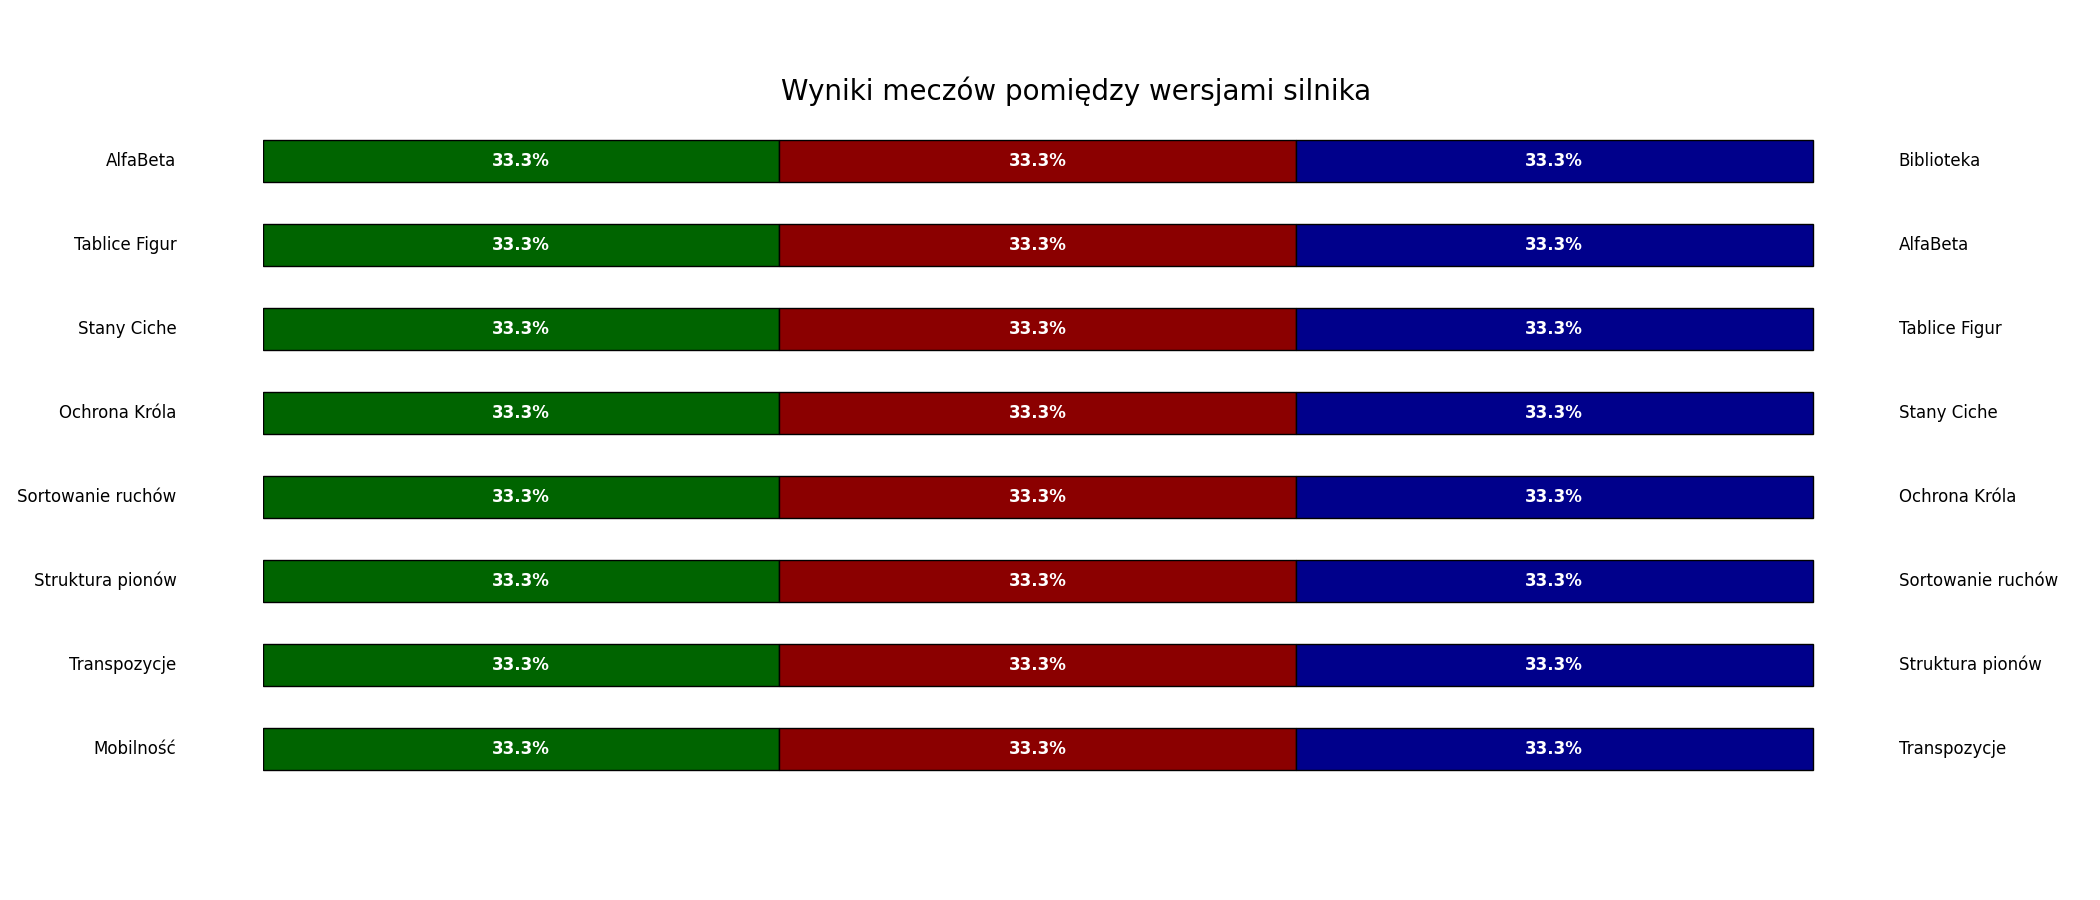
\includegraphics[width=1\linewidth]{rozdzialy/rozdzial03/1_porownanie-wersji-silnika/rysunki/gry-wyniki}
    \caption{Wyniki rozgrywek pomiędzy wersjami silnika}
    \label{fig:wyniki-wersje}
\end{figure}